%%%%%%%%%%%%%%%%%%%% author.tex %%%%%%%%%%%%%%%%%%%%%%%%%%%%%%%%%%%
%
% sample root file for your "contribution" to a proceedings volume
%
% Use this file as a template for your own input.
%
%%%%%%%%%%%%%%%% Springer %%%%%%%%%%%%%%%%%%%%%%%%%%%%%%%%%%


\documentclass{svproc}
%
% RECOMMENDED %%%%%%%%%%%%%%%%%%%%%%%%%%%%%%%%%%%%%%%%%%%%%%%%%%%
%

% to typeset URLs, URIs, and DOIs
\usepackage{url}
\usepackage[english]{babel}
\selectlanguage{english}
\usepackage[utf8]{inputenc}
\usepackage{graphicx}    % can use native umlauts
\usepackage[singlelinecheck=false]{caption}

\def\UrlFont{\rmfamily}

\begin{document}
\mainmatter              % start of a contribution
%
\title{Applying Machine Learning to Investigate Effects of contaminated PCR Plates in a Metagenomic Sequencing Study}
%
\titlerunning{Effects of contaminated PCR plates}  % abbreviated title (for running head)
%                                     also used for the TOC unless
%                                     \toctitle is used
%
\author{Maximilian Joas\inst{1} }
%
%\authorrunning{$<$Joas$>$ et al.} % abbreviated author list (for running head)
%
%%%% list of authors for the TOC (use if author list has to be modified)
\tocauthor{Maximilian Joas}
%
\institute{Universität Leipzig\\Machine Learning Group\\Leipzig, Germany\\
\email{mj13body@studserv.uni-leipzig.de}}
%
\maketitle              % typeset the title of the contribution
%
\begin{abstract}
 The objectives of this work are to predict contaminated PCR plates based on OTU read counts and to investigate specific characteristics of the contaminated plates. A random forest classifier and MLP were used to predict the plate as well as to find important characteristics of the contaminated plate. The prediction resulted in an accuracy of 0.84 and important OTUs had higher read counts than non-important ones. In conclusion, it is possible to predict contaminated PCR plates with machine learning based on OTU counts.
  \keywords{Machine Learning, Empirical Data, Scientific Research}
\end{abstract}
%
%
\section{Research Question}
%
Metagenomics an area of research that studies genetic material obtained directly from environmental samples.
Advances and cost reduction of sequencing experiments had a great impact on the field of Metagenomics \cite{junemann2017bioinformatics}.
The vast amount of data obtained from whole-genome sequencing experiments in metagenomic leads to opportunities in pathogen detection, ecological studies and drug development \cite{chiu2019clinical}\cite{junemann2017bioinformatics}. On the other hand, the abundance of data poses challenges to the analysis of metagenomic data. Consequently, classical statistical methods reach their limits and other approaches such as machine learning are often used \cite{Soueidan2017}.\\


Not only the amount of data but also the type of data are challenging, on top of that, the technical process of sequencing can lead to problems.
In particular, contamination and noise are important problems when studying metagenomics \cite{eisenhofer2019contamination}. Noised up and or contaminated data can lead to false conclusions in experiments. Therefore it would be valuable to predict contamination on PCR plates and find factors that are distinctive to contaminated PCR plates. In this work, I will investigate if it is possible to predict contaminated PCR plates based on OTU counts as well as metadata. Furthermore, I will present factors that distinguish contaminated from not contaminated PCR plates with the help of machine learning.


\section{State of the Art}
Machine learning methods have been successfully used in the study of metagenomics data  \cite{Soueidan2017}. A typical application is to use clustering algorithms to group barcode sequences into OTUs, in order to investigate the genetic diversity of a microbial community \cite{Soueidan2017}. Another use of machine learning is to analyze functional properties of microbial communities with the help of Hidden Markov Models or neuronal networks \cite{Soueidan2017}. However, specifically on this research question, there are, to the best of my knowledge no publications. The research questions can be modeled as typical machine learning problems as described in the following section.

%
%
\section{Methods}
%\subsection{Conception}

The research question is divided into two parts: (I) Is it possible to predict the contaminated PCR plate? (II) What did change on the contaminated PCR plates? \\
The first question is a typical problem for a supervised learning approach: I used two methods to predict the PCR Plate, one classical machine learning approach (Random Forest Classifier) and a neuro-inspired approach (Multi-Layer Perceptron).  Additionally, a dummy classifier and a decision tree classifier was used as a baseline.
In order to solve the second question in a machine learning context, the most important features for the supervised learning method were retrieved. Therefore, I had to use methods that not only predict the contaminated plate, but also determine the most important features for the prediction. The random forest Gini importance was used as a measurement, together with the Shapely value.
Both research questions have been examined with a dataset comprising of OTU count data and the corresponding metadata, which is presented in the following section.\\

%\subsection{Data and Preprocessing}

The data set was provided by the ETH Zurich. The data consisted of a count table of microorganisms sequencing reads from mice from different laboratories The data set did not come normalized. Additionally, to the count table, a data set containing metadata was included in the analysis. The metadata contained a variety of technical information, such as the PCR plate, the date of the extraction run, or the name of the researchers that executed the experiments. In total, the data set consisted of 199 samples and 1564 OTUs and 61 different metadata entries per sample. The median sequencing depth of the samples was 80275. Note that the ETH Zurich provided another dataset with three replicas of each sample, but for the analyses, the dataset without the replicas was used.\\
Firstly, 17 non-informative features, that had additionally an abundance of missing values, were excluded manually from the metadata. Subsequently, I aggregated the information about the PCR plate by grouping the not-contaminated plates together. This resulted in a binary classification problem. The count-table did not contain any missing values, the metadata had multiple features with missing values. When the metadata was used for the prediction, I excluded samples with missing values. 26 samples were excluded from this experiment. Subsequently, the datatype was checked, non-numeric data types were transformed to ordinal values. In contrast to one-hot encoding, this method does not increase the feature space. However, it can have an influence on the predictions.
For the count-table a z-transformation was performed, in order to use it for the multilayer perceptron.\\

%\subsection{Supervised Learning Methods}
In order to predict the contaminated class, the relative frequency of the more frequent class was established as a dummy classifier for comparison. Subsequently, a decision tree was used as a baseline classifier. In order to evaluate the decision tree, I used ten-fold cross-validation and Accuracy, Precision, Recall and F1 Score as the evaluation metric.
Subsequently, a random forest classifier was used to predict the contamination. Therefore the random forest classifier of scikit-learn v.0.23.2 \footnote{https://scikit-learn.org/stable/index.html} was implemented without tuning. The parameters can be found in Table 1. Since the latter two methods are statistically inspired, a neuro-inspired approach was used in addition. Herefore, a multilayer perceptron was implemented with the python package sckit-learn . The following parameters  were tuned with a grid search approach (grid parameters in brackets) and ten-fold cross validation: hidden layer size ((50,50,50), (50,100,50), (100,)), activation ("identity", "logistic", "tanh", "relu"), solver ("lbfgs", "sgd", "adam"), alpha (0.0001, 0.01, 0.05, 0.1) and learning rate ("constant","adaptive"). The number of maximum iterations was set to 500. All parameters are presented in Table 1.

\begin{table}
   \caption{Parameters of random forest classifier and MLP}
      \begin{center}
  % \begin{tabular*}{\columnwidth}{l @{\extracolsep{\fill{1}}}*{4}{l}@{l}}
  \begin{tabular*}{\textwidth}{l @{\extracolsep{\fill}} lllll}
   \hline
   Method & Parameter                        & Value       & Datatype\\ \hline
   Random Forest & n\_estimators                        & True       & boolean  \\
           & max\_features                             & auto     & String   \\
           & max\_samples\_leaf                            & 1     & int   \\
           & boostrap                           & True     & boolean   \\ \hline
   MLP   & hidden\_layer\_size                             & (50, 100, 50)       & tupel  \\
           & activation                       & tanh        & String     \\
           & solver                           & lbfgs  & String   \\
           & alpha & 0.0001      & float \\
           & learning\_rate                     & constant       & String      \\
         \hline
   \end{tabular*}
   \end{center}
\raggedright{\textbf{Note 1:} Default Paremeter Random Forest: $ccp_alpha: 0.0, class_weight: None, criterion: gini, max_depth: None, max_leaf_nodes: None, max_samples: None, min_impurity_decrease: 0.0, min_impurity_split: None, min_samples_split: 2, min_weight_fraction_leaf: 0.0, n_estimators: 200,  oob_score: False, random_state: 0.$}\\
{\raggedright \textbf{Note 2:} Default parameters MLP: $batch\_size: auto, beta\_1: 0.9, beta\_2: 0.999, early\_stopping: False, epsilon	1.00E-08, max\_fun:	15000, momentum: 0.9, n\_iter\_no\_change: 10, nesterovs\_momentum: True, power\_t: 0.5, random\_state: 1, shuffle	 True, adam, tol: 0.0001, validation\_fraction: 0.1.$ \par}

\end{table}

In order to answer the second research question - what was different on the contaminated plate -, the goal was to find features that are associated with the prediction of the contaminated plate. Therefore, the Gini importance of the random classifier was used. Additionally, the Shapley values of the features were calculated based on the trained random forest. The Shapely value is a metric for the contribution of a feature to the prediction \cite{roth1988shapley} \cite{2019contamination}. For the feature importance, the data was split with a stratified 70/30 ratio into training and test data. Finally, I used boxplots and beeswarmplot to descriptively analyze the difference between OTU counts of important and non-important features, in general, and across plates.
\section{Results}
The results of the two research questions are presented separately Firstly the results of the prediction of the PCR plate are presented.
\%subsection{Prediction of the PCR plate}
The dummy classifier, defined as the relative frequency of the more frequent class, was 0.52. Firstly, the results with the count data is presented: A decision tree served as a baseline classifier yielded an accuracy of $0.64\pm{0.14}$ after tenfold cross-validation.  The tenfold cross-validation of the random forest resulted in an average accuracy of $0.75\pm{0.10}$. The MLP beat the dummy classifier but had an average accuracy of $0.65\pm{0.13}$ almost no higher accuracy than the baseline decision tree classifier. Additional evaluation metrics like Precision, Recall and F1 score can be found in Table 2.\\
When using the metadata as features to predict the contaminated plate all evaluation metrics resulted in a perfect prediction (Accuracy:1, Precision:1, Recall:1, F1 score: 1).
\begin{table}
  \caption{Average evaluation metrics over all ten cross-validation runs, including the standard deviation, for the prediction of the PCR plate}
  \begin{center}
   
      \begin{tabular*}{\textwidth}{l @{\extracolsep{\fill}} lllll}
          \hline
       
                 Method & Accuracy & Precision & Recall & F1 Score\\[2pt]
                                  \hline\rule{0pt}{12pt}Decision Tree  &    0.64$\pm{0.14}$ & 0.67$\pm{0.12}$ & 0.61$\pm{0.26}$ & 0.57$\pm{0.18}$ \\
                  Random Forest &    0.75$\pm{0.10}$ & 0.83$\pm{15}$ & 0.66$\pm{0.28}$  & 0.68$\pm{0.20}$  \\
                  MLP    &    0.65$\pm{0.13}$ &  0.64$\pm{0.17}$  & 0.63$\pm{0.28}$ & 0.60$\pm{0.19}$ \\
                  [2pt]
                  \hline
      \end{tabular*}
  \end{center}
\end{table}


%\subsection{Features of the contaminated PCR plate}
In order to investigate differences between contaminated and non-contaminated plates, the ten most important features according to the random forest Gini importance were extracted for the count data and the metadata.  Since there were no notable differences between the Shapley value and the Gini importance, only results of the Gini importance are reported.
The most important metadata features were the date of the 16S PCR, the extraction run and the library prep attempt. The ten most important OTUs are classified as follows: unclassified Bacteroidales OTU(72), unclassified Lachnospiraceae (OTU 257), Lachnospiraceae UCG-006 OTU(385), Lachnospiraceae NK4A136 group (OTU 207), Enterorhabdus OTU(296), Blautia OTU(803), unclassified Bacteroidales OTU(68), Lactobacillus OTU(102), unclassified Lachnospiraceae OTU(311), unclassified Bacteroidales OTU(514).
Figures 1A and 1B show a beeswarmplot of counts of the ten most (Fig. 1A) and ten least important (Fig. 1B) features. Figures 1A and 1B show that the least important features have a higher count number for the outlier samples. Figures 1C and 1D show the boxplots of the counts of the most (Fig. 1C) and least (Fig. 1D) important features. The median differences in count numbers do not reveal a clear trend. Figures 1E and 1F compare the counts of contaminated and non-contaminated samples of the most (Fig. 1E) and least(Fig.1F) important OTUs.

\begin{figure}
		
		
		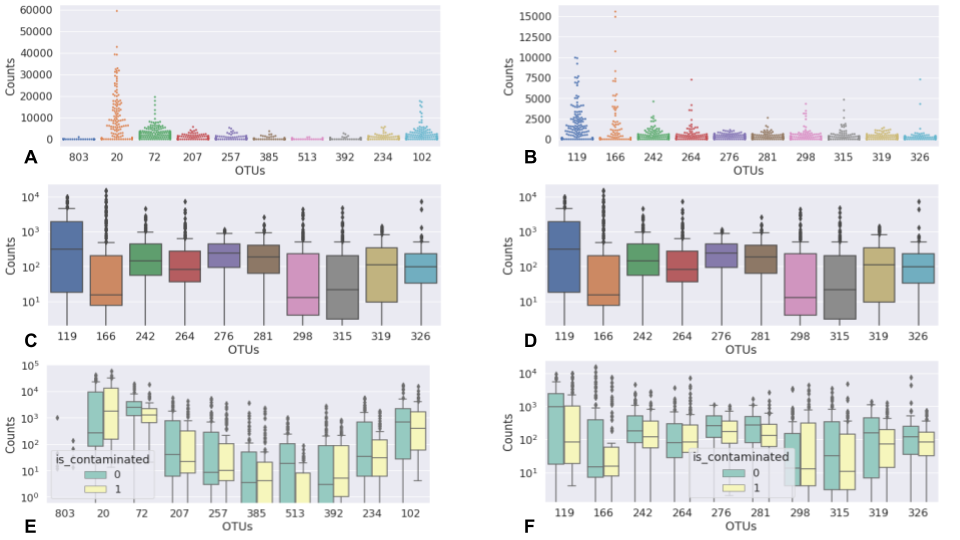
\includegraphics[ width=1\textwidth]{./figs/plotsPraktikum.png}
		\caption{\textbf{A and B}: Beeswarmplot of counts of the ten most (A) and ten lead (B) important OTUs according to Gini importance. \textbf{C and D}: Boxplot of of counts of the ten most (C) and ten least (D) important OTUs. \textbf{E and F}: Boxplots of counts of contaminated and non-contaminated samples of most (E) and least (F) important OTUs}
	\end{figure}
\section{Discussion}
The results of the prediction of the PCR plates seem plausible for the analyses with the count data. The results as shown in Table 2 reveal that a more complex MLP is not superior to the simple decision tree. However, when using statistically inspired models the complex random forest is superior to the decision tree in all metrics. The comparatively small value of the recall of the random forest classifier implies a higher number of false negatives. Since the presented analyses were highly specific to the data and question there are not existing reference metrics from other publications. However, in a general machine learning context, the results are reasonable. The lack of tuning for the random forest could be seen as a major limitation of this work. However, the predictions resulted in accurate predictions and could therefore be used to extract important features even without tuning.
The fact that the prediction with the metadata yielded perfect predictions seems highly unplausible at first sight. On the other hand, the information about the PCR plate of the sample could be encoded in other metadata features. e.g plate one was performed on certain days. This could also be observed when contemplating the feature importance where the date of the 16s PCR step was the most important feature.
The analyses of the OTU importance showed that important OTUs had less extreme count numbers for their outlier samples, which is counterintuitive. There was also no trend that the important features had higher median count numbers than the non-important ones. This is unexpected because one could argue that the contamination needs to be somehow visible for instance through higher count numbers. Consequently, contaminated plates should have higher count numbers. The comparison between OTU counts of contaminated and non-contaminated samples for the important and least important OTUs did allow to draw any conclusions. Descriptive statistics could be the wrong method to investigate differences between important and non-important OTUs due to the high dimensionality of the data. Thus, unsupervised machine learning approaches like clustering could have been useful.
On the other hand, only a fraction of all OTUs were analyzed, hence a comparison of the 100 most and least important OTUs could reveal differences.
In general, it is hard to draw a causal conclusion about specific contaminations, because I assumed the samples were distributed randomly across the PCR plates, which is not generally the case.
\section{Conclusion}
%
In summary, it is possible to predict the contaminated plate with the OTU count data. A random forest classifier yields the most accurate predictions but has a comparatively high false-negative rate. Additionall, OTUs were found that predicted the contaminated plate particularly well.Hence there could be found a difference between contaminated and non-contaminated PCR plates: No meaningfuls differences in the count numbers of important and non-important OTUs were found. It remains subject to future research, relevant OTUs for the prediction of the contaminated plate have a different count profile than non-informative OTUs. In this work machine learning and a neuro-inspired approach were used. A comparison with a Bayesian approach could be interesting in further studies.

%
% ---- Bibliography ----
%
%
\bibliographystyle{plain}
\bibliography{Paperrunde.bib}


\end{document}





